%% LyX 2.0.5.1 created this file. For more info, see http://www.lyx.org/.
%% Do not edit unless you really know what you are doing.
%\documentclass[10pt]{beamer}\usepackage{graphicx, color}
%% maxwidth is the original width if it is less than linewidth
%% otherwise use linewidth (to make sure the graphics do not exceed the margin)
\makeatletter
\def\maxwidth{ %
  \ifdim\Gin@nat@width>\linewidth
    \linewidth
  \else
    \Gin@nat@width
  \fi
}
\makeatother

\IfFileExists{upquote.sty}{\usepackage{upquote}}{}
\definecolor{fgcolor}{rgb}{0.2, 0.2, 0.2}
\newcommand{\hlnumber}[1]{\textcolor[rgb]{0,0,0}{#1}}%
\newcommand{\hlfunctioncall}[1]{\textcolor[rgb]{0.501960784313725,0,0.329411764705882}{\textbf{#1}}}%
\newcommand{\hlstring}[1]{\textcolor[rgb]{0.6,0.6,1}{#1}}%
\newcommand{\hlkeyword}[1]{\textcolor[rgb]{0,0,0}{\textbf{#1}}}%
\newcommand{\hlargument}[1]{\textcolor[rgb]{0.690196078431373,0.250980392156863,0.0196078431372549}{#1}}%
\newcommand{\hlcomment}[1]{\textcolor[rgb]{0.180392156862745,0.6,0.341176470588235}{#1}}%
\newcommand{\hlroxygencomment}[1]{\textcolor[rgb]{0.43921568627451,0.47843137254902,0.701960784313725}{#1}}%
\newcommand{\hlformalargs}[1]{\textcolor[rgb]{0.690196078431373,0.250980392156863,0.0196078431372549}{#1}}%
\newcommand{\hleqformalargs}[1]{\textcolor[rgb]{0.690196078431373,0.250980392156863,0.0196078431372549}{#1}}%
\newcommand{\hlassignement}[1]{\textcolor[rgb]{0,0,0}{\textbf{#1}}}%
\newcommand{\hlpackage}[1]{\textcolor[rgb]{0.588235294117647,0.709803921568627,0.145098039215686}{#1}}%
\newcommand{\hlslot}[1]{\textit{#1}}%
\newcommand{\hlsymbol}[1]{\textcolor[rgb]{0,0,0}{#1}}%
\newcommand{\hlprompt}[1]{\textcolor[rgb]{0.2,0.2,0.2}{#1}}%

\usepackage{framed}
\makeatletter
\newenvironment{kframe}{%
 \def\at@end@of@kframe{}%
 \ifinner\ifhmode%
  \def\at@end@of@kframe{\end{minipage}}%
  \begin{minipage}{\columnwidth}%
 \fi\fi%
 \def\FrameCommand##1{\hskip\@totalleftmargin \hskip-\fboxsep
 \colorbox{shadecolor}{##1}\hskip-\fboxsep
     % There is no \\@totalrightmargin, so:
     \hskip-\linewidth \hskip-\@totalleftmargin \hskip\columnwidth}%
 \MakeFramed {\advance\hsize-\width
   \@totalleftmargin\z@ \linewidth\hsize
   \@setminipage}}%
 {\par\unskip\endMakeFramed%
 \at@end@of@kframe}
\makeatother

\definecolor{shadecolor}{rgb}{.97, .97, .97}
\definecolor{messagecolor}{rgb}{0, 0, 0}
\definecolor{warningcolor}{rgb}{1, 0, 1}
\definecolor{errorcolor}{rgb}{1, 0, 0}
\newenvironment{knitrout}{}{} % an empty environment to be redefined in TeX

\usepackage{alltt}
\setcounter{secnumdepth}{3}
\setcounter{tocdepth}{3}
\usepackage{url}
\ifx\hypersetup\undefined
  \AtBeginDocument{%
    \hypersetup{unicode=true,pdfusetitle,
 bookmarks=true,bookmarksnumbered=false,bookmarksopen=false,
 breaklinks=false,pdfborder={0 0 0},backref=false,colorlinks=false}
  }
\else
  \hypersetup{unicode=true,pdfusetitle,
 bookmarks=true,bookmarksnumbered=false,bookmarksopen=false,
 breaklinks=false,pdfborder={0 0 0},backref=false,colorlinks=false}
\fi
\usepackage{breakurl}

\makeatletter

%%%%%%%%%%%%%%%%%%%%%%%%%%%%%% LyX specific LaTeX commands.
\providecommand{\LyX}{\texorpdfstring%
  {L\kern-.1667em\lower.25em\hbox{Y}\kern-.125emX\@}
  {LyX}}

%%%%%%%%%%%%%%%%%%%%%%%%%%%%%% Textclass specific LaTeX commands.
 % this default might be overridden by plain title style
 \newcommand\makebeamertitle{\frame{\maketitle}}%
 \AtBeginDocument{
   \let\origtableofcontents=\tableofcontents
   \def\tableofcontents{\@ifnextchar[{\origtableofcontents}{\gobbletableofcontents}}
   \def\gobbletableofcontents#1{\origtableofcontents}
 }
 \def\lyxframeend{} % In case there is a superfluous frame end
 \long\def\lyxframe#1{\@lyxframe#1\@lyxframestop}%
 \def\@lyxframe{\@ifnextchar<{\@@lyxframe}{\@@lyxframe<*>}}%
 \def\@@lyxframe<#1>{\@ifnextchar[{\@@@lyxframe<#1>}{\@@@lyxframe<#1>[]}}
 \def\@@@lyxframe<#1>[{\@ifnextchar<{\@@@@@lyxframe<#1>[}{\@@@@lyxframe<#1>[<*>][}}
 \def\@@@@@lyxframe<#1>[#2]{\@ifnextchar[{\@@@@lyxframe<#1>[#2]}{\@@@@lyxframe<#1>[#2][]}}
 \long\def\@@@@lyxframe<#1>[#2][#3]#4\@lyxframestop#5\lyxframeend{%
   \frame<#1>[#2][#3]{\frametitle{#4}#5}}

%%%%%%%%%%%%%%%%%%%%%%%%%%%%%% User specified LaTeX commands.
%\usetheme{PaloAlto}
  \usetheme{Warsaw}
%  %\usetheme{default}
  \setbeamercovered{invisible}

\makeatother

\begin{document}






%\makebeamertitle

\lyxframeend{}
%
%
%\AtBeginSection[] % Do nothing for \section*
{
\begin{frame}<beamer>
\frametitle{}
\tableofcontents[currentsection] % Inhaltsverz. vor jeder Section einblenden
\end{frame}
}
%\mode<presentation>
%{
\title {Dynamic Transit times and mean ages}
\subtitle {Applications to non steady state scenarios} % (optional)
\author {Markus Müller, Carlos Sierra}
\makebeamertitle
%
%%%%%%%%%%%%%%%%%%%%%%%%%%%%%%%%%%%%%%%%%%%%%%%%%%%%%%%%%%%%%%%%%%%%%%%%%%%%%%%%%%%%%%%%%%%%%%%%%%%%%
\begin{frame}
  \titlepage
\end{frame}
\begin{frame}
  \frametitle{Outline}
  \tableofcontents[pausesections]
\end{frame}
%%%%%%%%%%%%%%%%%%%%%%%%%%%%%%%%%%%%%%%%%%%%%%%%%%%%%%%%%%%%%%%%%%%%%%%%%%%%%%%%%%%%%%%%%%%%%%%%%%%%%
%%%%%%%%%%%%%%%%%%%%%%%%%%%%%%%%%%%%%%%%%%%%%%%%%%%%%%%%%%%%%%%%%%%%%%%%%%%%%%%%%%%%%%%%%%%%%%%%%%%%%
\section{Introduction}
%%%%%%%%%%%%%%%%%%%%%%%%%%%%%%%%%%%%%%%%%%%%%%%%%%%%%%%%%%%%%%%%%%%%%%%%%%%%%%%%%%%%%%%%%%%%%%%%%%%%
%%%%%%%%%%%%%%%%%%%%%%%%%%%%%%%%%%%%%%%%%%%%%%%%%%%%%%%%%%%%%%%%%%%%%%%%%%%%%%%%%%%%%%%%%%%%%%%%%%%%
\begin{frame}
\frametitle{The general concept of a reservoir}
  %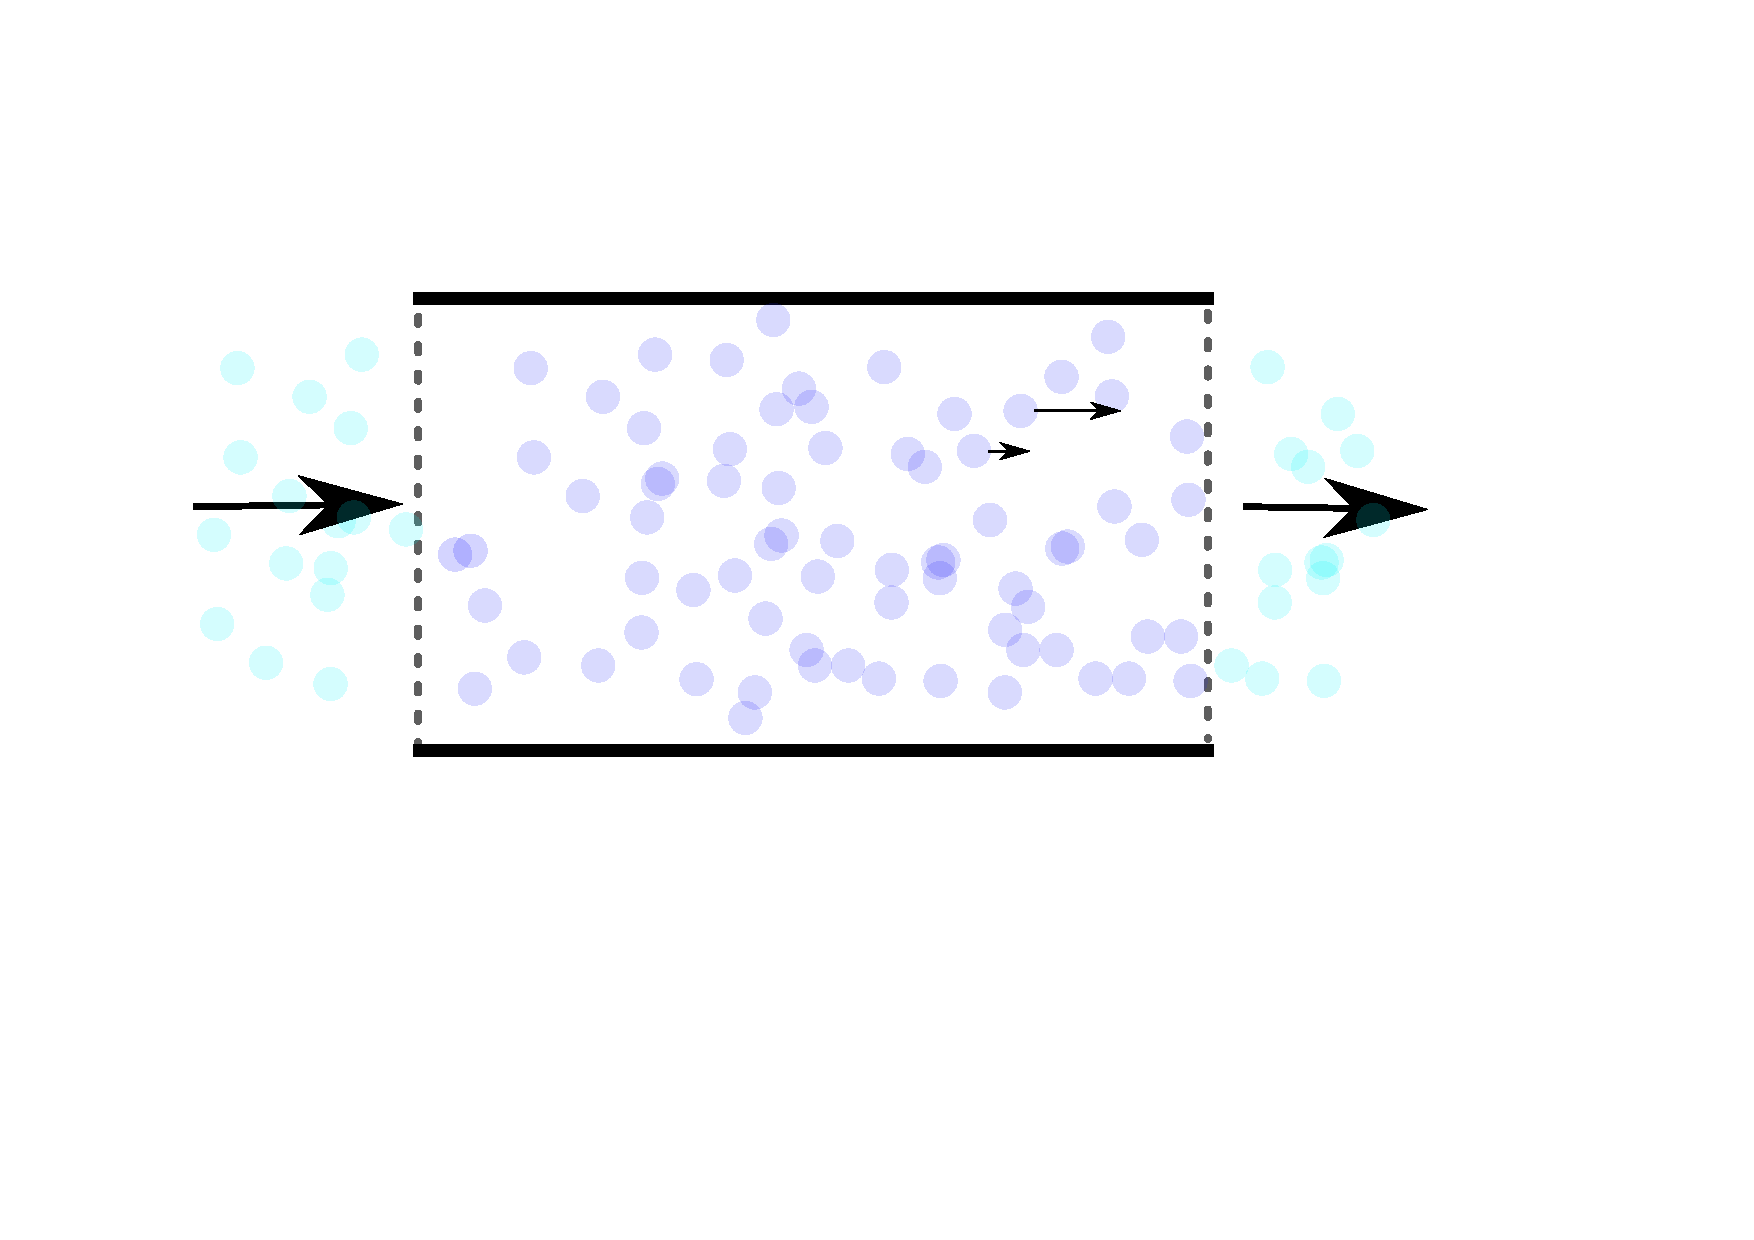
\includegraphics[height=0.8\textheight]{Reservoir.pdf}
  \includegraphics<1>[width=0.6\textwidth]{Reservoir.pdf}
  \includegraphics<2>[width=0.6\textwidth]{Reservoir_People.pdf}
\begin{enumerate}
\item <2>in and out ``flows'' do not necessarily involve ``movement'' 
\item <2>in and out flow ``channels'' do not always have to be defined physically or spatially 
\end{enumerate}
\note<1>{Imagine a reservoir of particles with an input and an output channel. 
Particles will enter the system through some input channel, will stay there for a while and eventually leave the system through an output stream. 
Here Only the dark blue particles are ``in'' the reservoir. 
}
\note<2>{
Although the concept of a reservoir is usually intuitively attached to some kind of a pool with fluid moving trough it 
the idea is more general. 

An example that shows how generally this idea can be applied is the human population of the world.
A particle here refers to a human beeing that is born, lives and dies.

The inflow and outflow boundaries are not spatially defined in this case 
}

\end{frame}
%%%%%%%%%%%%%%%%%%%%%%%%%%%%%%%%%%%%%%%%%%%%%%%%%%%%%%%%%%%%%%%%%%%%%%%%%%%%%%%%%%%%%%%%%%%%%%%%%%%%%
\begin{frame}
\frametitle{age of a particle}
  \includegraphics<1,2>[width=0.6\textwidth]{ParticleAge.pdf}
  \note<1>{
  We can define the age of a particle with respect to the reservoir as the time it has spent in it.
  In the case of the human population this refers to the age in common sense.
  But in general the age refers not to the time of creation but to the time the reservoir was entered.
  If the reservoir in question is e.g. the soil and the particle a $^{14}C$ atom that entered the soil 5 minutes ago
  it is at least 
  possible that the atom is as old as the universe while its age with respect to the soil is only 5 minutes}
  
\begin{itemize}
     \item <2> The ``age '' is always defined in \emph{context} of the reservoir
\end{itemize}

\end{frame}
%%%%%%%%%%%%%%%%%%%%%%%%%%%%%%%%%%%%%%%%%%%%%%%%%%%%%%%%%%%%%%%%%%%%%%%%%%%%%%%%%%%%%%%%%%%%%%%%%%%%%
\begin{frame}
 [fragile]
\frametitle{Mean age }
\begin{itemize}
   \item Usually time dependent
   \item Includes \emph{all} particles that are in the reservoir at the given time.
   \item Usually depends on input rates as well as the dynamics of the system.
\end{itemize}
%\begin{tabular}{tt}
  \includegraphics<1>[width=0.6\textwidth]{Reservoir_Peoples_Ages.pdf}
  \[
  \bar a(t) =\frac{a_1+a_2+\cdots+a_N}{N}
  \]
  With $N=N(t)$ the number of all particles in the reservoir at time $t$.
%\end{tabular}
  \note{To compute the average age of the population  of the world at a given time we would have to ask everybody how old he is and then compute the mean value.
  If we treat this room as a reservoir everybody would have started a stopwatch entering the room, press the stop botton now and we would have to add all the times and divide them by the number of people.}
\end{frame}
%%%%%%%%%%%%%%%%%%%%%%%%%%%%%%%%%%%%%%%%%%%%%%%%%%%%%%%%%%%%%%%%%%%%%%%%%%%%%%%%%%%%%%%%%%%%%%%%%%%%%
\begin{frame}
 [fragile]
\frametitle{Mean transit time }
  \includegraphics<1>[width=0.6\textwidth]{MeanTransitTime.pdf}
  \[
  \bar t_r(t) =\frac{a_1+a_2+\cdots+a_{NO}}{NO}
  \]
  With $NO=NO(t)$ the number of particles {\color{red} just leaving} at time $t$
\begin{itemize}
   \item Can be time dependent as well
   \item Includes only the subset of particles that are just leaving at the given time.
   (Can only be computed when there is an output stream)
   \item could be independent of input rates and only depend on the dynamics of the system.
\end{itemize}
\note{In the example of the world population it would be sufficient to observe the grave yards.
We would investigate the birth date of every person who dies and compute the average of the live spans. We ignore all the people still alive and concentrate only on the people just dying.
In this room it would be hard to compute the average transit time right now, because nobody is leaving at the moment. (dropping of to sleep does not count as leaving).
But we could after the talk.
Every person would press the stop bottom at its watch in the moment she passes the door.
If two or more people would leave in the same moment we could compute the average of the
times. }
\end{frame}
%%%%%%%%%%%%%%%%%%%%%%%%%%%%%%%%%%%%%%%%%%%%%%%%%%%%%%%%%%%%%%%%%%%%%%%%%%%%%%%%%%%%%%%%%%%%%%%%%%%%%
\begin{frame}
 [fragile]
\frametitle{Comparison}
\begin{tabular}{cc}
  \includegraphics<1>[width=0.5\textwidth]{Reservoir_Peoples_Ages.pdf} 
  &
  \includegraphics<1>[width=0.5\textwidth]{MeanTransitTime.pdf}
\end{tabular}
\end{frame}
%%%%%%%%%%%%%%%%%%%%%%%%%%%%%%%%%%%%%%%%%%%%%%%%%%%%%%%%%%%%%%%%%%%%%%%%%%%%%%%%%%%%%%%%%%%%%%%%%%%%%
%\begin{frame}
%\frametitle{Confusing Definitions}
%\begin{tabular}{|c|c|c|}
%\hline
%Source &   Name 	& Definition \\
%\hline
%%Example text outside R code here; we know the value of pi is pi.
%\end{tabular}
%\end{frame}
%%%%%%%%%%%%%%%%%%%%%%%%%%%%%%%%%%%%%%%%%%%%%%%%%%%%%%%%%%%%%%%%%%%%%%%%%%%%%%%%%%%%%%%%%%%%%%%%%%%%%
%
%%%%%%%%%%%%%%%%%%%%%%%%%%%%%%%%%%%%%%%%%%%%%%%%%%%%%%%%%%%%%%%%%%%%%%%%%%%%%%%%%%%%%%%%%%%%%%%%%%%%
\begin{frame}
 [fragile]
\frametitle{Example Model}
  \includegraphics<1>[width=0.9\textwidth]{LasagaModel.pdf}
\end{frame}
%%%%%%%%%%%%%%%%%%%%%%%%%%%%%%%%%%%%%%%%%%%%%%%%%%%%%%%%%%%%%%%%%%%%%%%%%%%%%%%%%%%%%%%%%%%%%%%%%%%
\begin{frame}
 [fragile]
\frametitle{Didactical Considerations}

\makebox[0pt][l]{
  \includegraphics<1>[width=0.9\textwidth]{LasagaModelTransp.pdf}
  \includegraphics<2>[width=0.9\textwidth]{LasagaModelTranspEquation.pdf}
  \includegraphics<3>[width=0.9\textwidth]{LasagaModelTranspEquationLast.pdf}
  \includegraphics<4>[width=0.9\textwidth]{LasagaModelTranspEquationLastWithParts.pdf}
  \includegraphics<5>[width=0.9\textwidth]{LasagaModelTranspEquationLastWithPartsImputOutput.pdf}
}
\raisebox{5cm}{
\begin{minipage}{10cm}
   \begin{itemize}
      \item<1,2,3>
      The system is a \emph{cycle}. \\ 
      $\rightarrow$ Nothing leaves the system as a whole. \\
      $\rightarrow$ Transit times for the whole system do not make sense.\\
      $\rightarrow$ We will observe sub reservoirs \\
      \item<2,3> 
	 We want to demonstrate a usecase not accessible with analytic methods. \\
	 $\rightarrow$ we will perturb the system out of its steady state.
	 Fortunately \emph{all} equations are nonlinear. So there is no chance to
	 compute anything without a numerical method.
      \item <3> We do not want to complicate matters unnecessaryly.\\
      $\rightarrow$ We will go for the simplest equation.\\
      $\rightarrow$ observe the last pool.\\
   \end{itemize}
\end{minipage}
}
\end{frame}
%%%%%%%%%%%%%%%%%%%%%%%%%%%%%%%%%%%%%%%%%%%%%%%%%%%%%%%%%%%%%%%%%%%%%%%%%%%%%%%%%%%%%%%%%%%%%%%%%%%%%%
\begin{frame}
 [fragile]
\frametitle{Mean transit time for the last pool}
\begin{itemize}
   \item<1,2> remember:
   \begin{enumerate}
      \item
         To compute the mean transit time we have to identify the particles {\color{red} just leaving}.
      \item
         Ask every leaving  particle   when it entered and compute its age.
      \item
         Iterate over all particle and compute the average of their ages.
     \[
     \bar t_r(t) =\frac{a_1+a_2+\cdots+a_{NO}}{NO}
     \]
     With $NO=NO(t)$ the number of particles just leaving at time $t$
   \end{enumerate}
  \item<2>Equivalent method: Iterate over all ages and ask how many particles are of that age. (histogram)
\begin{enumerate}
   \item as above
   \item as above + make a histogram of all ages
   \item iterate over all ages and compute their weighted average
     \[
     \bar t_r(t) =\frac{a_1 n_{a_1} +a_2 n_{a_2} +\cdots+a_{n}n_{a_n}}{NO}
     \]
     With $NO=NO(t)=n_{a_1} + n_{a_2} +\cdots +n_{a_n}$ 
   \end{enumerate}
\end{itemize}
  %\includegraphics<1>[width=0.9\textwidth]{LasagaModel.pdf}
\end{frame}
%%%%%%%%%%%%%%%%%%%%%%%%%%%%%%%%%%%%%%%%%%%%%%%%%%%%%%%%%%%%%%%%%%%%%%%%%%%%%%%%%%%%%%%%%%%%%%%%%%%%%%
\begin{frame}
[fragile]
\frametitle{Second Test}
Text is nice but let's see what happens if we make a couple of plots
in our chunk:
\begin{knitrout}\footnotesize
\definecolor{shadecolor}{rgb}{0.969, 0.969, 0.969}\color{fgcolor}\begin{kframe}
\begin{alltt}
\hlfunctioncall{par}(las = 1, mar = \hlfunctioncall{c}(4, 4, 0.1, 0.1))  \hlcomment{# tick labels direction}
\hlfunctioncall{boxplot}(x)
\hlfunctioncall{hist}(x, main = \hlstring{""}, col = \hlstring{"blue"}, probability = TRUE)
\hlfunctioncall{lines}(\hlfunctioncall{density}(x), col = \hlstring{"red"})
\end{alltt}
\end{kframe}

{\centering 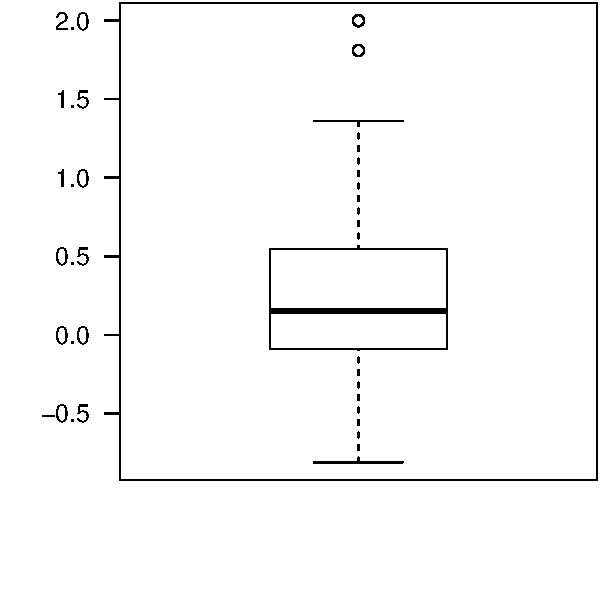
\includegraphics[width=.45\linewidth]{figure/beamer-boring-plots1} 
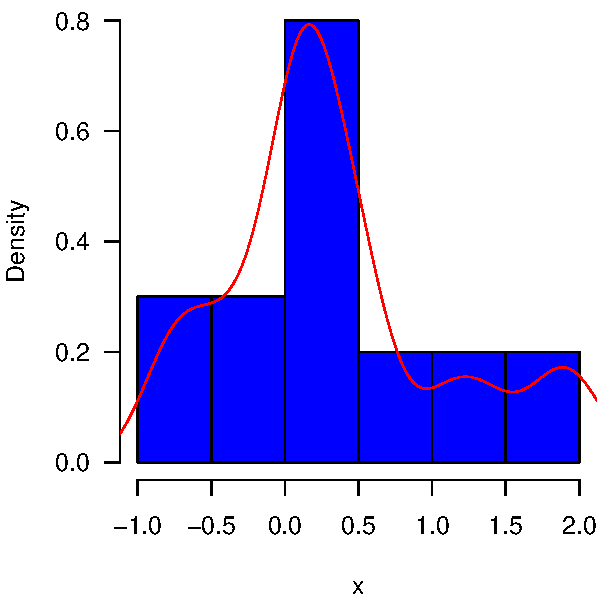
\includegraphics[width=.45\linewidth]{figure/beamer-boring-plots2} 

}



\end{knitrout}

\end{frame}
%%%%%%%%%%%%%%%%%%%%%%%%%%%%%%%%%%%%%%%%%%%%%%%%%%%%%%%%%%%%%%%%%%%%%%%%%%%%%%%%%%%%%%%%%%%%%%%%%%%%%%
%\begin{frame}
%[fragile]
%\frametitle{Python}
%Now we proudly present a python script that uses sympy to produce the latex part.
%<<mm,echo=FALSE,eval=TRUE,engine='python',results="asis">>=
%from meanage import *
%lp(dic["sol_abstract"])
%lp(dic["sol_constant"])
%@
%\end{frame}
%%%%%%%%%%%%%%%%%%%%%%%%%%%%%%%%%%%%%%%%%%%%%%%%%%%%%%%%%%%%%%%%%%%%%%%%%%%%%%%%%%%%%%%%%%%%%%%%%%%%%
%\begin{frame}
% [fragile]
%\frametitle{}
%\end{frame}
\end{document}
